\documentclass[article]{jss}
\usepackage[utf8]{inputenc}

\providecommand{\tightlist}{%
  \setlength{\itemsep}{0pt}\setlength{\parskip}{0pt}}

\author{
Jane Analyst\\Prestigious University \And Joe Postdoc\\Slightly less prestigious school
}
\title{Was Ty Cobb a better hitter than Babe Ruth?}
\Keywords{Sabermetrics, Cobb, Ruth}

\Abstract{
We use Bayesian analysis to establish the likelihood that one batter was
better than another.
}

\Plainauthor{Jane Analyst, Joe Postdoc}
\Plaintitle{Was Ty Cobb a better hitter than Babe Ruth?}
\Plainkeywords{sabermetrics, cobb, ruth}

%% publication information
%% \Volume{50}
%% \Issue{9}
%% \Month{June}
%% \Year{2012}
\Submitdate{}
%% \Acceptdate{2012-06-04}

\Address{
    Jane Analyst\\
  Prestigious University\\
  13 Ivy Lane Collegeville, USA\\
  E-mail: \href{mailto:Jane@FancySchool.com}{\nolinkurl{Jane@FancySchool.com}}\\
  URL: \url{http://www.fancySchool.com}\\~\\
    }

\usepackage{amsmath}

\begin{document}

Did Ty Cobb hit better than the Babe? Let's use Bayesian analysis to try
and find out!

The graph below is a posterior density of each player's batting average
using an uninformed beta prior density.

\begin{CodeChunk}


\begin{center}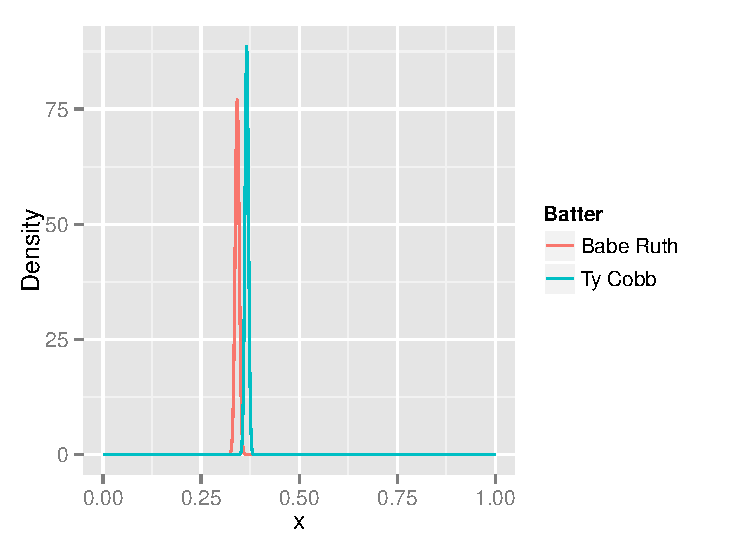
\includegraphics{Demo_files/figure-latex/unnamed-chunk-2-1} \end{center}

\end{CodeChunk}

Looks like Ty Cobb was a better hitter.

\end{document}

